% !TeX spellcheck = de_CH_frami

\section{MOS-Diode (Kap. 7)}
Um eine MOS-Diode aus einem MOS-Transistor zu erhalten, werden die Anschlüsse von Gate und Drain verbunden.\\ 
\begin{tabular}{|p{0.11\textwidth}|p{0.14\textwidth}|p{0.16\textwidth}|p{0.145\textwidth}|p{0.125\textwidth}|p{0.2\textwidth}|}
	\hline
	\multicolumn{2}{|c|}{\textbf{Reale Diode:}}&\multicolumn{4}{c|}{\textbf{MOS-Diode:}}\\ \hline
	Symbol&Kennlinie&N-MOS-Diode&P-MOS-Diode&Kennlinie&KS-Ersatzschaltung\\
	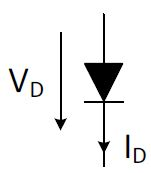
\includegraphics[height=2.6cm]{chapters/Diode/images/realeDiode}&
	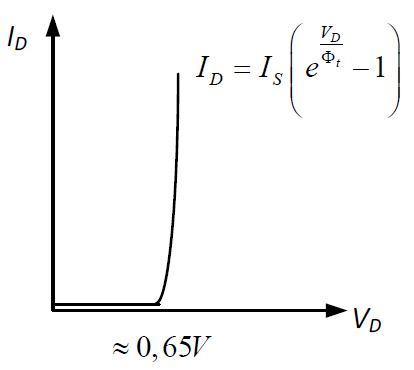
\includegraphics[height=2.6cm]{chapters/Diode/images/KennlinieRealeDiode}&
	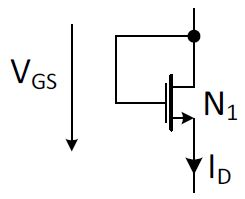
\includegraphics[height=2.6cm]{chapters/Diode/images/NMOS-Diode}&
	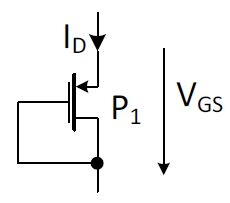
\includegraphics[height=2.6cm]{chapters/Diode/images/PMOS-Diode}&
	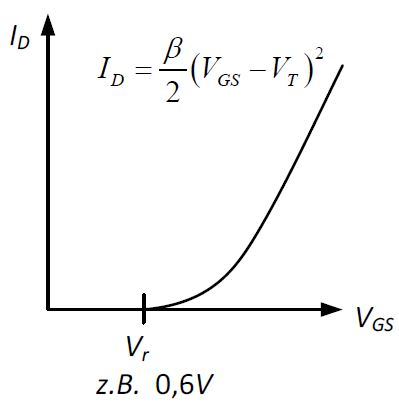
\includegraphics[height=2.6cm]{chapters/Diode/images/KennlinieDiode}&
	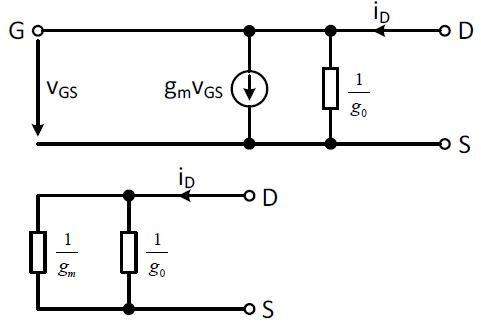
\includegraphics[height=2.6cm]{chapters/Diode/images/KS_Diode}\\ \hline
\end{tabular}\\[1ex]
\begin{tabular}{|l|l|}
	\hline
	Arbeitspunktstrom einer MOS-Diode mit Widerstandslast $R_D$&$I_D=\frac{\beta}{2}(V_{GS}-V_T)^2\textcolor{gray}{(1+\lambda V_{DS})} = \frac{V^+-V_{GS}}{R_D}$\\ \hline
	$V_{DS}$ einer MOS-Diode bei gegebenem Strom&$V_{DS}=V_T + \sqrt{\frac{2I_D}{\beta \textcolor{gray}{(1+\lambda V_{DS})}}}\approx V_T + \sqrt{\frac{2I_D}{\beta}}$\\ \hline
	Innenwiderstand der MOS-Diode&$r_{MD}=\frac{v_{GS}}{i_D}=\frac{1}{g_m+g_0}\approx\frac{1}{g_m}$\\ \hline
	Im quadratischen Bereich gilt:&$g_m=\beta(V_{GS}-V_T)=\sqrt{2\beta I_D}$\\ \hline
\end{tabular}\\ [1ex]
Bei der leitenden MOS-Diode ist der Transistor immer gesättigt, weil $V_{DS}>V_{DS,sat} = (V_{GS}-V_T)$ jederzeit erfüllt ist.
\textbf{MOS-Dioden als Spannungsteiler}\\
\begin{tabular}{|p{0.2\textwidth}|p{0.25\textwidth}|p{0.2\textwidth}|p{0.25\textwidth}|}
	\hline
	\textbf{Mit Bodyeffekt}&\textbf{Ohne Bodyeffekt}&\multicolumn{2}{l|}{\textbf{Mehrfach Spannungsteiler}}\\ \hline
	$V_{SB1}=0$, $V_{SB2}=V_{GS1}$ daher Body-Effekt und $V_{T2} > V_{T1}$&$V_{SB1}=0$,$V_{SB2}=0$ daher kein Body-Effekt. Es gelten die Nominalwerte für $V_{T2}$, $V_{T1}$&Lokales Substrat, $V_{Ti}$ für alle gleich $\rightarrow$ gleiche Teilspannungen&Gemeinsames Substrat, unterschiedliche $V_{Ti}$ $\rightarrow$ unterschiedliche Teilspannungen\\
	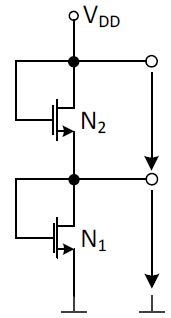
\includegraphics[height=2.6cm]{chapters/Diode/images/SpgT_N_Bodyeffekt}&
	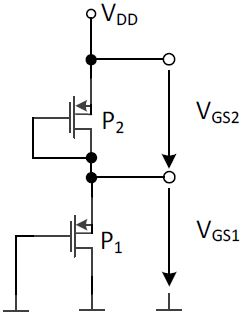
\includegraphics[height=2.6cm]{chapters/Diode/images/SpgT_P_body}
	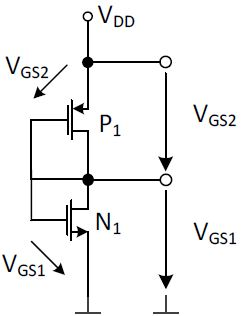
\includegraphics[height=2.6cm]{chapters/Diode/images/SpgT_PN}&
	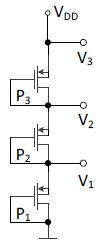
\includegraphics[height=2.6cm]{chapters/Diode/images/SpgT_P3}&
	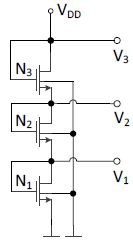
\includegraphics[height=2.6cm]{chapters/Diode/images/SpgT_N3}\\    
	\hline	
\end{tabular} \\ [1ex]
Verhältnis: $\frac{|V_{GS1}-V_{T1}|}{|V_{GS2}-V_{T2}|}=\sqrt{\frac{\beta_2}{\beta_1}}=\sqrt{\frac{(W/L)_2\beta_{02}}{{(W/L)_1\beta_{01}}}$